%%%%%%%%%%%%%%%%%%%%% Chapter 7 %%%%%%%%%%%%%%%%%%%%%%%%%%%%%%%%%
% Federated Learning: Decentralized Intelligence
%%%%%%%%%%%%%%%%%%%%%%%%%%%%%%%%%%%%%%%%%%%%%%%%%%%%%%%%%%%%%%%%%
\motto{``Your data stays on your device. Only model updates are shared.'' This is the promise of Federated Learning, but it is also where the hidden risks begin.}

\chapter{Federated Learning: Decentralized Intelligence}
\label{chap:federated_learning}

\abstract{Federated Learning (FL) has emerged as the leading architecture for collaborative AI without data centralization. However, as this chapter demonstrates, the mere decentralization of data does not guarantee privacy. We explore the core mechanisms of Federated Learning, analyze the "Privacy Illusion" created by raw gradient sharing, and introduce the combined framework of DP-FL. We specifically address the challenges of Non-IID data and communication overhead, drawing on optimizations for resource-constrained Fog and edge infrastructure.}

\section{The Federated Promise}
\label{sec:federated_promise}

Traditional AI training requires moving all raw data into a single centralized server---a massive, vulnerable honeypot for attackers and a regulatory nightmare for architects. \textbf{Federated Learning (FL)} \cite{mcmahan2017} fundamentally changes this pattern. It allows multiple clients (such as hospitals, banks, or mobile devices) to train a global model collaboratively without ever sharing their raw records \cite{science-journal}.

For industries like healthcare, the promise is transformative: ten hospitals can train a state-of-the-art disease prediction model while ensuring that no patient's private history ever leaves the local hospital firewalls.

\section{The FL Architecture: Local Training and Global Aggregation}
\label{sec:fl_architecture}

In a standard Federated Learning loop (often using the \textbf{FedAvg} algorithm \cite{mcmahan2017}), the process follows four repeating steps:

\begin{enumerate}
    \item \textbf{Broadcasting:} The global server sends the current model weights to selected clients.
    \item \textbf{Local Training:} Each client trains the model on its local, private data.
    \item \textbf{Update Submission:} Clients send only the model's weight updates (gradients) back to the server.
    \item \textbf{Aggregation:} The server aggregates the updates (typically via weighted averaging) to improve the global model.
\end{enumerate}

\begin{figure}[t]
\centering
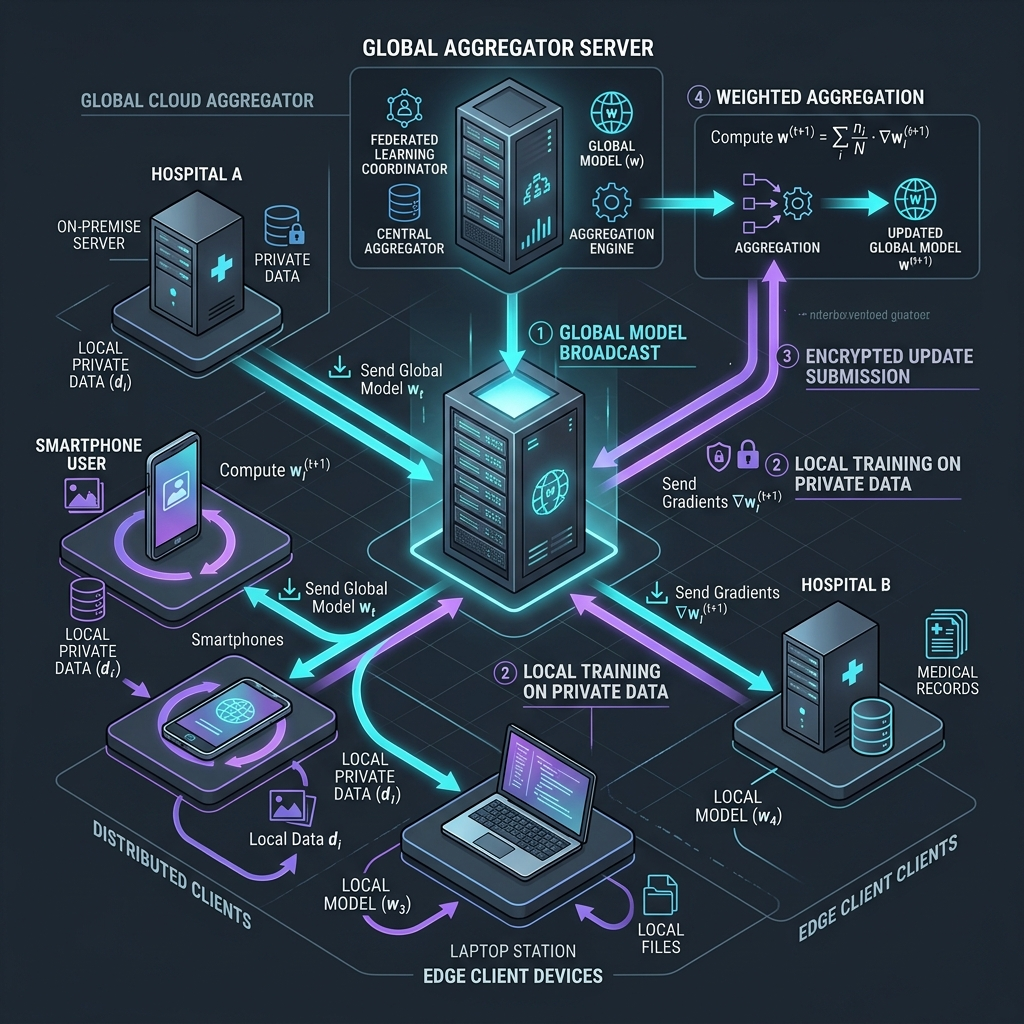
\includegraphics[width=\textwidth]{figures/ch7_fl_arch.png}
\caption{The Federated Learning Architecture: Illustrating the global model broadcast, local edge training, and subsequent aggregation of model updates without raw data movement.}
\label{fig:ch7_fl_arch}
\end{figure}

\section{The Privacy Illusion: Why FL Alone Is Not Enough}
\label{sec:privacy_illusion}

Despite the decentralization of raw data, Federated Learning alone is not inherently privacy-preserving. Research has shown that these shared model gradients can be reverse-engineered through \textbf{Gradient Inversion Attacks} \cite{zhu2019}, effectively reconstructing the original training images or records from the numerical updates.

\begin{table}
\caption{Primary Risks in Standard Federated Learning}
\label{tab:fl_risks}
\begin{tabular}{p{3cm}p{5cm}p{2cm}}
\hline\noalign{\smallskip}
Risk Type & Mechanism & Impact \\
\noalign{\smallskip}\svhline\noalign{\smallskip}
Gradient Inversion & Adversary reconstructs data from shared updates. & \textcolor{red}{$\bullet$} High \\
Membership Inference & Determining if an individual was in a client's set. & \textcolor{orange}{$\bullet$} Medium \\
Model Poisoning & Malicious clients corrupting the global weights. & \textcolor{red}{$\bullet$} High \\
\noalign{\smallskip}\hline\noalign{\smallskip}
\end{tabular}
\end{table}

\section{The Solution: DP-FL}
\label{sec:dp_fl}

To turn the "Privacy Illusion" into a concrete guarantee, the Trustworthy AI Architect must combine Federated Learning with \textbf{Differential Privacy (DP-FL)}. By having each client clip their gradients and add calibrated Gaussian noise before submission, we ensure that no individual record's signal can be extracted from the global aggregate.

\section{Real-World Challenges: Overhead and Stability}
\label{sec:fl_challenges}

Implementing DP-FL in the wild introduces two major bottlenecks:

\begin{description}
  \item[Communication Overhead:] 
        Sending high-dimensional updates frequently consumes massive bandwidth. In the \textbf{POP2TIC} framework \cite{science-DOI}, we found that by optimizing the compression and noise strategies, overhead can be reduced by up to 40 percent without compromising the $\epsilon$-guarantee.
  \item[Non-IID Data:]
        In many real-world settings, data is not "Independent and Identically Distributed" (Non-IID) across clients. A hospital in a rural area may have significantly different data than one in an urban center, making global convergence difficult when combined with DP noise.
\end{description}

\section{Conclusion}
\label{sec:conclusion_fl}

Federated Learning provides the architectural scaffolding for decentralized trust, but it requires the mathematical shield of DP and the cryptographic protection of \textbf{Secure Aggregation} to be fully secure. In the next chapter, we look at how to protect the update process itself from a curious or compromised central server.


